 
\documentclass{article}
\title{\textbf{7. MĚŘENÍ ROZPTYLOVÉHO MAGNETICKÉHO POLE TRANSFORMÁTORU}}
\author{Tomáš Kysela}
\date{21/3/2022}

\addtolength{\topmargin}{-3cm}
\addtolength{\textheight}{3cm}

\usepackage[czech]{babel}
\usepackage{graphicx}
\usepackage{circuitikz}
\usepackage{amsmath}
\usepackage{subcaption}
\usepackage{pgfplots}
\usepackage{siunitx}
\usepackage{multirow}
\usepackage{pgfplots}
\usepackage{tabularx}
\usepackage{parskip}
\usepackage{float}
\sisetup{detect-all}

\makeatletter
\providecommand\add@text{}
\newcommand\tagaddtext[1]{%
	\gdef\add@text{#1\gdef\add@text{}}}%
\renewcommand\tagform@[1]{%
	\maketag@@@{\llap{\add@text\quad}(\ignorespaces#1\unskip\@@italiccorr)}%
}
\makeatother

\begin{document}
	
	\maketitle
	
	\section{Úkol měření}
		\begin{enumerate}
			\item Určete potřebné parametry měřící cívky: konstantu $K_{CH}$, vlastní rezonanční úhlový kmitočet $\omega_r$ a hodnoty prvků $L_s$ a $C_p$ paralelního náhradního schématu.
			\item Změřte rozptylové magnetické pole transformátoru. Měření proveďte ve vodorovné rovině procházející středním sloupkem transformátoru.
			\item Z výsledků měření určete, v jaké vzdálenosti lze pole transformátoru považovat za pole dipólového charakteru.
		\end{enumerate}
	\section{Schéma zapojení}
	\begin{figure}[H]
		\centering
		\begin{circuitikz}[european]
			\ctikzset{american inductors}
			\draw (0,1.0) to[twoport,t=$G$] (0,-1.0);
			\draw (1,1.0) to[rmeter,t=$mA$] (3,1.0);
			\draw (4,1.0) to[twoport,t=$V$] (4,-1.0);
			\draw (6,2.0) to[L,l=$L_s$] (8,2.0);
			\draw (8,2.0) to[R,l=$R_s$] (10,2.0);
			\draw (7,0) to[C,l=$C_p$] (9,0);
			\draw (0,1.0) to[short] (1,1.0);
			\draw (3,1.0) to[short] (5,1.0);
			\draw (5,1.0) to[short] (5,2.0);
			\draw (5,2.0) to[short] (6,2.0);
			\draw (5,1.0) to[short] (5,-0.0);
			\draw (5,-0.0) to[short] (7,-0.0);
			\draw (9,-0.0) to[short] (11,-0.0);
			\draw (11,1.0) to[short] (11,-0.0);
			\draw (10,2.0) to[short] (11,2.0);
			\draw (11,2.0) to[short] (11,1.0);
			\draw (11,1.0) to[short] (12,1.0);
			\draw (12,1.0) to[short] (12, -1.0);
			\draw (12, -1.0) to[short] (0, -1.0);
			\draw (7,-1.0) node[rground]{};
		\end{circuitikz}
	\caption{Obvod pro stanovení vlastního rezonančního kmitočtu}
	\end{figure}
\begin{figure}[H]
	\centering
	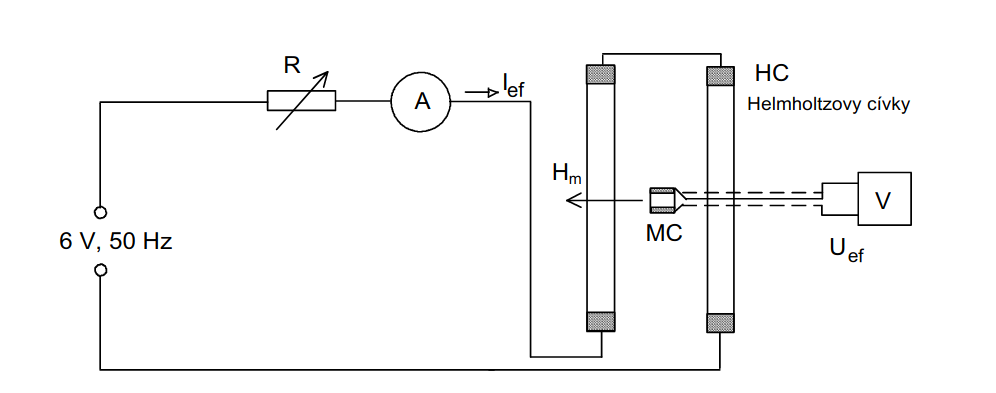
\includegraphics[width=0.7\linewidth]{screenshot001}
	\caption{Obvod pro stanovení konstanty měřicí cívky}
	\label{fig:screenshot001}
\end{figure}

\section{Soupis použitých přístrojů}
\begin{tabular}{ll}
	$G$ & RC generátor, typ GFG-8020H \\
	$T_r$ & transformátor jako zdroj měřeného rozptylového pole \\
	$V$ & nf voltmetr, typ TVT-321 \\
	$mA$ & miliampérmetr, tř.přes. 1.5 , rozsah 2 \si{\ampere} \\
	$HC$ & Helmholtzovy cívky, $K_{HZ} = 276 \si{\ampere\per\meter}$ \\
	$MC$ & měřicí cívka\\
\end{tabular}

\section{Teoretický základ}

Pro periodické průběhy s jedním průchodem nulou během periody lze magnetickou indukci 
vypočítat ze vztahu

\begin{equation}
	B_m = \frac{U_s}{4fSN} \tagaddtext{[\si{\tesla}]}
\end{equation}
kde $B_m$ je maximální hodnota složky měřené indukce $B(t)$, $U_s$ aritmetická střední hodnota napětí $U(t)$ (po dvoucestném usměrnění) 
indukovaného v měřicí cívce, $f$ kmitočet základní harmonické měřeného napětí, $N$ počet závitů měřicí cívky a $S$ plocha průřezu měřicí cívky.

Maximální hodnotu intenzity magnetického pole $H_m$ vypočítáme ze vztahu
\begin{equation}
	H_m = \frac{B_m}{\mu_0}
\end{equation}
Budeme-li napětí indukované v měřicí cívce měřit voltmetrem udávajícím hodnotu $U_ef$ získanou měřením střední hodnoty $U_s$ po dvoucestném usměrnění a násobením činitelem tvaru $1.11$ pro sinusový průběh, můžeme hodnotu $U_s$ získat vydělením údaje přístroje $1.11$. (Pozor, pro neharmonický průběh neodpovídá údaj efektivní hodnotě).

\subsection{Měřený objekt}
V některých případech lze zdroj magnetického pole, jehož siločáry se uzavírají převážně vzduchem, přibližně nahradit polem magnetického dipólu (viz obr. 3).
\begin{figure}[H]
	\centering
	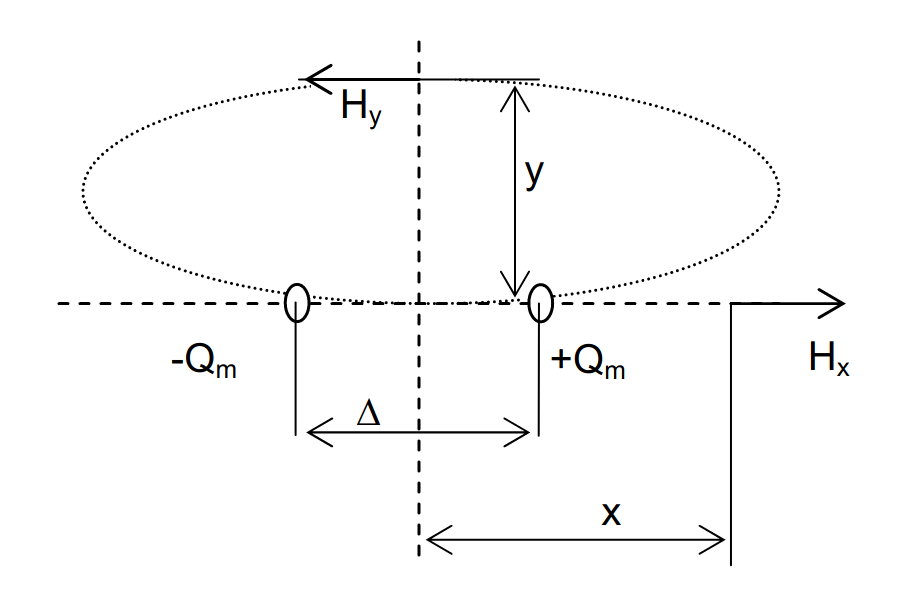
\includegraphics[width=0.6\linewidth]{screenshot002}
	\caption{Souřadnicový systém pro měření dipólového pole v rovině $xy$}
	\label{fig:screenshot002}
\end{figure}

Za předpokladu, že $\Delta<<x$ resp. $y$, lze intenzitu magnetického pole v rovině $xy$ na osách $x$ a $y $ vyjádřit vztahy
\begin{equation}
	H_x = \frac{m_C}{2\pi\mu_0x^3}, H_y = \frac{m_C}{4\pi\mu_0y^3}
\end{equation}
kde $m_C$ je Coulombův magnetický moment, $\mu_0$ je magnetická konstanta (permeabilita vakua) a $x,y$ jsou vzdálenosti měřených bodů od středu dipólu.

ze-li měřením složek $H_x$ a $H_y$ dokázat, že v určité vzdálenosti od měřeného objektu má magnetické pole dipólový charakter, je v této oblasti zcela určeno hodnotou $m_C$ .

\subsection{Určení parametrů měřicí cívky}
Odpor vinutí cívky $R_S = 8.15\si{\kilo\ohm}$(lze určit libovolnou stejnosměrnou metodou). Celkovou 
impedanci cívky změříme např. Ohmovou metodou. Předem musíme ale znát hodnotu vlastního rezonančního kmitočtu  fr  cívky, který zjistíme např. měřením v zapojení podle 
obr. 1. Obvod  je  napájen  ze  zdroje  konstantního  napětí  $U$.  Při  rezonančním  kmitočtu    $f_r$  ,  kdy  je  impedance cívky maximální, je proud  $I$  minimální. Platí
\begin{equation}
	f_r = \frac{1}{2\pi\sqrt{L_sC_p}}
\end{equation}

Impedanci měřicí cívky měříme při  $f_m = 0.1 f_r$ , kdy je vliv  $C_p$  zanedbatelný. Pro impedanci při kmitočtu  $f_m$  platí

\begin{equation}
	Z_m = \frac{U_m}{I_m} = \sqrt{R_s^2+\omega_m^2L_s^2}, L_s = \frac{1}{\omega_m}\sqrt{Z_m^2-R_s^2}
\end{equation}
kde $U_m$ je napětí měřené při kmitočtu  $f_m$ , $I_m$  je proud měřený při kmitočtu  $f_m$ . Hodnotu $C_p$ vypočteme ze vztahu (4), kde známe změřený rezonanční kmitočet $f_r$ a indukčnost $L_s$. 

\subsection{Určení konstanty měřicí cívky}
Konstantu  $K_{CH}$  měřicí cívky určíme ve známém poli Helmholtzových cívek v zapojení podle obr. 2. Protože magnetické pole cívek má stejnou frekvenci (50 \si{\hertz}) a stejný průběh (harmonický) jako rozptylové pole transformátoru, platí
\begin{equation}
	K_{CH} = \frac{H_{max}}{U_{ef}} = \frac{\sqrt{2}I_{ef}K_{HZ}}{U_{ef}}
\end{equation}
kde  $K_{HZ}$  je konstanta Helmholtzových cívek, 
$I_{ef}$  je proud Helmholzových cívek a $U_{ef}$ je napětí indukované v měřicí cívce.

\subsection{Měření intenzity rozptylového pole transformátoru }
Měření rozptylového magnetického pole transformátoru provedeme v uspořádání dle obr. 4.
\begin{figure}[H]
	\centering
	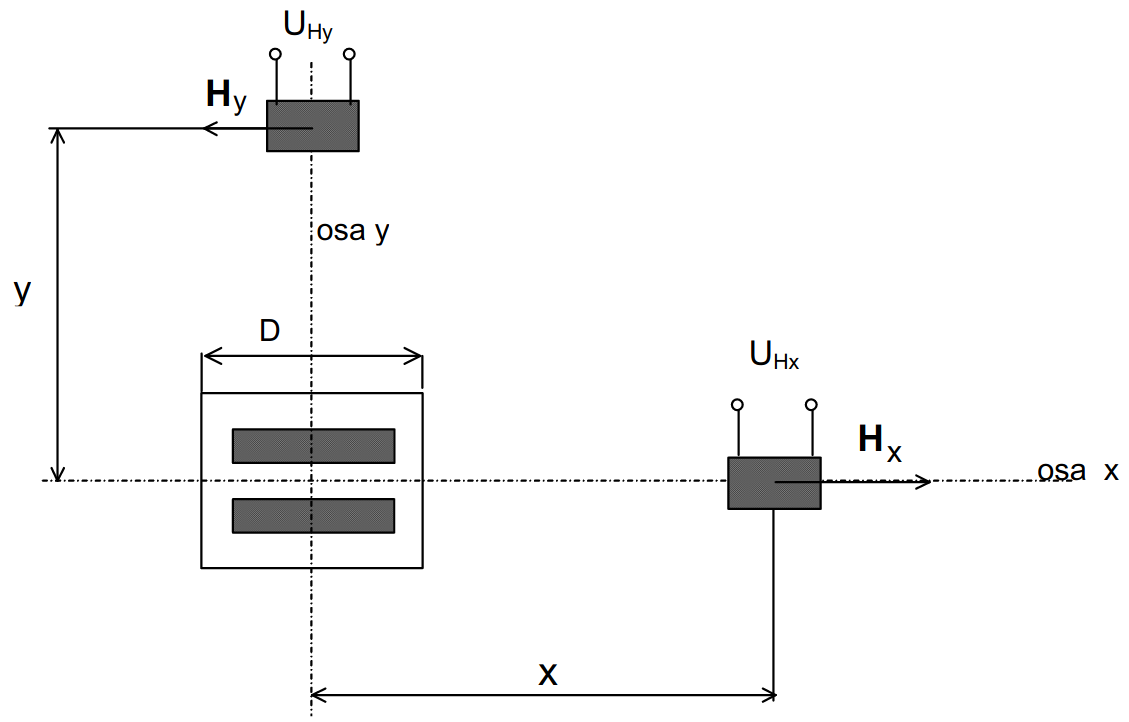
\includegraphics[width=0.6\linewidth]{screenshot003}
	\caption{Umístění sondy pro měření rozptylového pole}
	\label{fig:screenshot003}
\end{figure}
V několika vzdálenostech na osách $x$ a $y$ od středu transformátoru změříme napětí indukovaná v měřicí cívce a s využitím vztahu (6) vypočteme hodnoty  intenzity  $H_{xmax} =  K_{CH}\cdot U_{Hx} = f(x)$  a  $H_{ymax} = K_{CH}\cdot U_{Hy} = f(y)$.  Z naměřených hodnot vypočteme podle (3) $m_C$ a zjistíme, v jakých vzdálenostech měřené pole odpovídá poli dipólového charakteru ( $m_C = $konst).

\section{Naměřené hodnoty}
\subsection{Určení parametrů cívky}
$$
\begin{aligned}
	f_m &= 346.8 \si{\hertz}\\
	U_m &= 6.4 \si{\volt}\\
	I_m &= 0.58 \si{\milli\ampere}\\
	\\
	Z_m &= \frac{U_m}{I_m} = \frac{6.4 \si{\volt}}{0.58 \si{\milli\ampere}} = 11034.5 \si{\ohm}\\
	\omega_m &= 2\pi f_m = 2\pi \cdot 346.8 \si{\hertz} = 2179.01 \si{\per\second}\\
	L_s &= \frac{1}{\omega_m}\sqrt{Z_m^2-R_s^2}=\frac{1}{2179.01 \si{\per\second}}\sqrt{(11034.5 \si{\ohm})^2-(8150\si{\kilo\ohm})} = 3.41389 \si{\henry}\\
	\\
	f_r &= 10 \cdot f_m = 3468 \si{\hertz}\\
	C_p &= \frac{1}{4\pi^2f_r^2L_s} = \frac{1}{4\pi^2(3468 \si{\hertz})^2\cdot3.41389 \si{\henry}}=0.616925\si{\nano\farad}\\
	\\
	I_{ef} &= 1 \si{\ampere}\\
	U_{ef} &= 0.6 \si{\volt}\\
	K_{CH} &= \frac{\sqrt{2}I_{ef}K_{HZ}}{U_{ef}} = \frac{\sqrt{2}\cdot 1 \si{\ampere} \cdot 276 \si{\ampere\per\meter}}{0.6 \si{\volt}} = 650.538 \si{\ampere\per\meter\per\volt}
\end{aligned}
$$

\subsection{Rozptylové magnetické pole transformátoru}
Výpočet $H_{x/y}$ a $m_c$:
$$
\begin{aligned}
	H_{x/y} &= U_{Hx/Hy} \cdot K_{CH}\\
	m_c &= H_x \cdot 2 \cdot \pi \cdot \mu_0 \cdot x^3 = H_y \cdot 4 \cdot \pi \cdot \mu_0 \cdot y^3\\
	\mu_0 &= 1.25663706212 \cdot 10^{-6} \si{\henry\per\meter}
\end{aligned}
$$
\begin{figure}[H]
	\centering
		\begin{tabular}{c|c||c|c}
			$x [\si{\centi\meter}]$ & $U [\si{\milli\volt}]$ & $H_x [\si{\ampere\per\meter}]$ & $m_c [\si{\tesla\meter\cubed}]$ \\\hline \hline
			20 &46.0 &29.925 &1.890 \\\hline
			25 &22.2 &14.442 &1.782 \\\hline
			30 &16.8 &10.929 &2.330 \\\hline
			35 &8.4 &5.465 &1.850 \\\hline
			40 &5.4 &3.513 &1.775 \\\hline
			45 &3.6 &2.342 &1.685 \\\hline
			50 &3.0 &1.952 &1.926 \\\hline
			55 &2.4 &1.561 &2.051 \\\hline
			60 &2.0 &1.301 &2.219 \\\hline
			65 &1.6 &1.041 &2.257 \\\hline
			70 &1.4 &0.911 &2.467 \\\hline
			75 &1.2 &0.781 &2.600 \\\hline
			80 &1.0 &0.651 &2.630 \\\hline
			85 &0.8 &0.520 &2.524 \\\hline
			90 &0.8 &0.520 &2.996 \\\hline
			95 &0.8 &0.520 &3.523 \\\hline
			100 &0.6 &0.390 &3.082
		\end{tabular}
	\end{figure}
\begin{figure}[H]
	\centering
		\begin{tabular}{c|c||c|c}
			$y [\si{\centi\meter}]$ & $U [\si{\milli\volt}]$ & $H_y [\si{\ampere\per\meter}]$ & $m_c [\si{\tesla\meter\cubed}]$ \\\hline \hline
			10 &144.0 &93.677 &1.479 \\\hline
			15 &46.0 &29.925 &1.595 \\\hline
			20 &19.2 &12.490 &1.578 \\\hline
			25 &10.2 &6.635 &1.637 \\\hline
			30 &6.0 &3.903 &1.664 \\\hline
			35 &3.6 &2.342 &1.586 \\\hline
			40 &3.0 &1.952 &1.972 \\\hline
			45 &1.8 &1.171 &1.685 \\\hline
			50 &1.8 &1.171 &2.311
		\end{tabular}
\end{figure}
\subsection{Závěr}
Ve směru osy x a y se nejvyšší a nejnižší hodnota liší přibližně o $1 \si{\tesla\meter\cubed}$, což je natolik malá změna, že se dá prohlásit, že pole má všude dipólový charakter.
\end{document}
